\chapter{Metodologia}

	
    TROCAR PROPOSTA, AGORA JÀ È UMA METODOLOGIA
    A proposta deste trabalho é avaliar a testabilidade de um SMA utilizando o Moise como modelo de organização e empregando rede de Petri como ferramenta de descrição e análise. Em \cite{winikoff2014testability} e \cite{winikoff2017bdi} um grafo de controle de fluxo foi utilizado para avaliar a testabilidade de um sistema BDI. Partindo como base o trabalho de \cite{winikoff2017bdi} o grafo de controle de fluxo apresentado na Figura \ref{fig:control_fluxo} foi transformado em uma RP Figura \ref{fig:cf_rp}.

\begin{figure}[ht]
\centering
\includegraphics[scale=0.4]{imagens/fig18.png}
\caption{RP do grafo de controle de fluxo.}
\label{fig:cf_rp}
\end{figure}
    
  EXPLICANDO O PASSO A PASSO A AÇÃO A1 VIROU O LUGAR A1 A TRANSAÇÃO T1 REPRESENTA UM N E A TRANSAÇÃO T6 REPRESENTA O Y. EXPLICAR A5 = N E COMO CONTA OS CAMINHOS NA REDE DE PETRI


  

  
  A EF no nível individual é representado pelas missões, e no nível coletivo pelos Esquemas Sociais (ES). Um ES é essencialmente uma árvore de decomposição de metas globais. Um ES para o exemplo proposto é representando na Figura \ref{fig:es_exemplo}.
  
%\begin{figure}[ht]
%\centering
%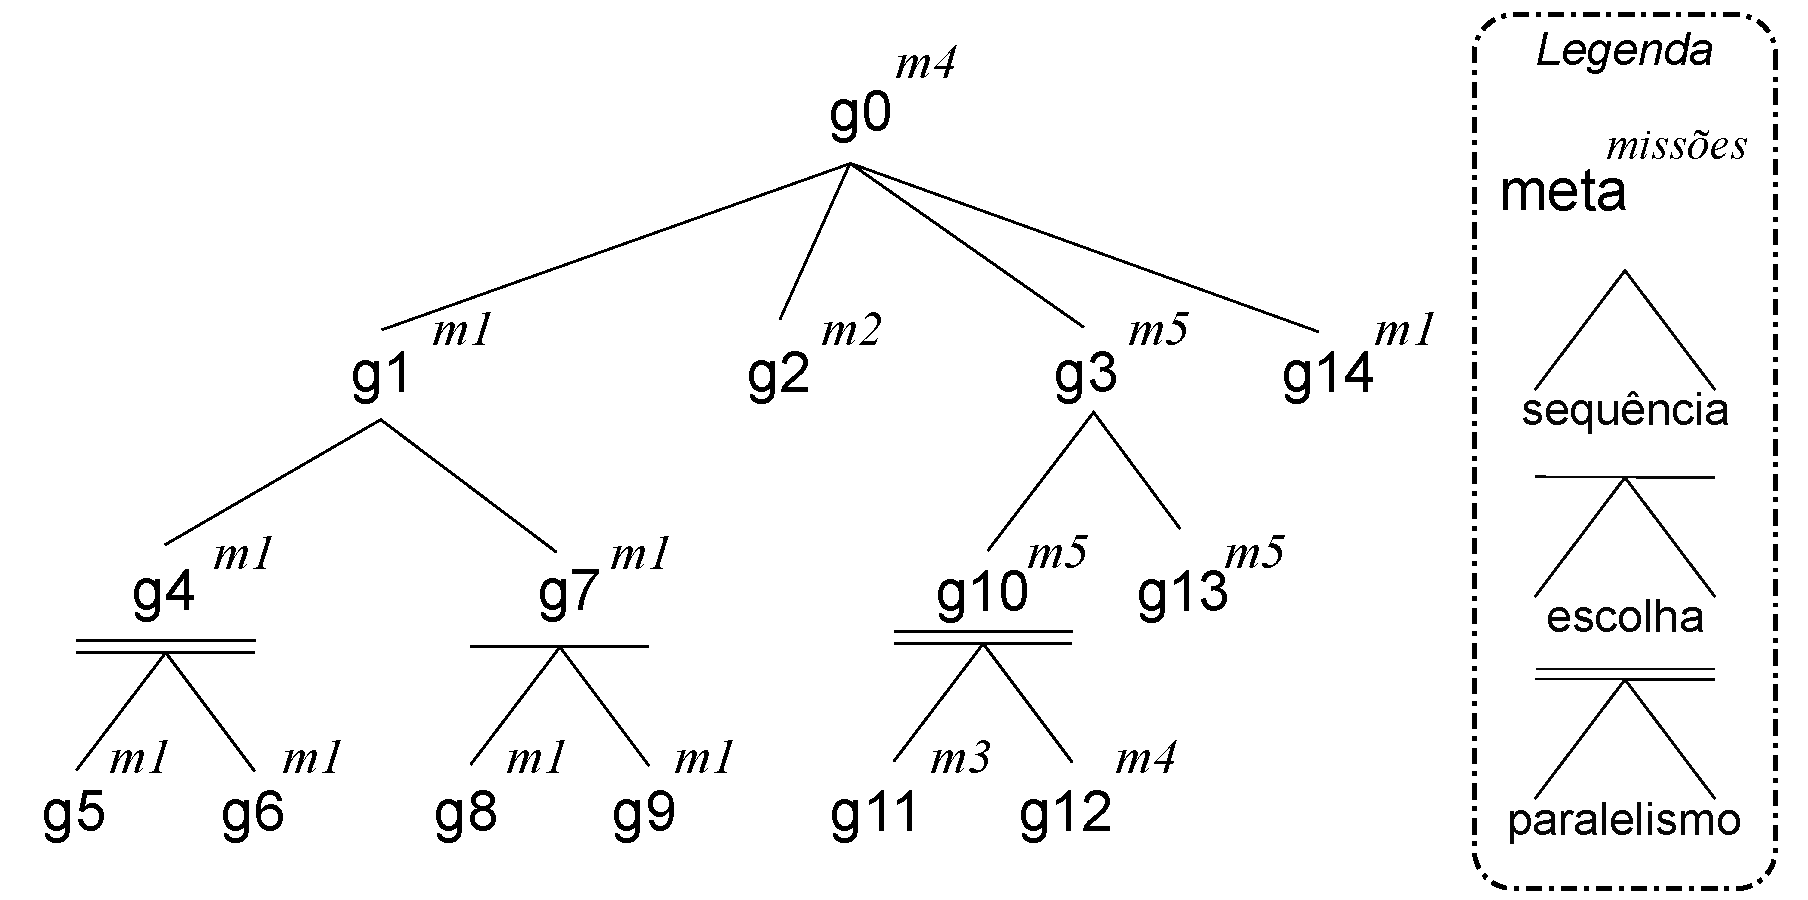
\includegraphics[scale=0.35]{imagens/ES2.png}
%\caption{Esquema Social para o exemplo \cite{hubner2003modelo}.}
%\label{fig:es_exemplo}
%\end{figure}






Assim através da árvore de metas globais é transformada em uma RP de acordo para cada missão Figura %\ref{fig:missoes_rp}.


%\begin{figure}[ht]
%\centering
%\includegraphics[scale=1]{imagens/RPGoals.pdf}
%\caption{Transformação das missões do exemplo em RP.}
%\label{fig:missoes_rp}
%\end{figure